\section{Optimizing}

\subsection{Restrictions}
As a reminder: $L$ is the length of the robot, and $w$ the width of the flywheel cylinders.
\begin{enumerate}
\item Not crashing with the ground at any inclination can be translated as:
\begin{figure}[ht]
	\centering
	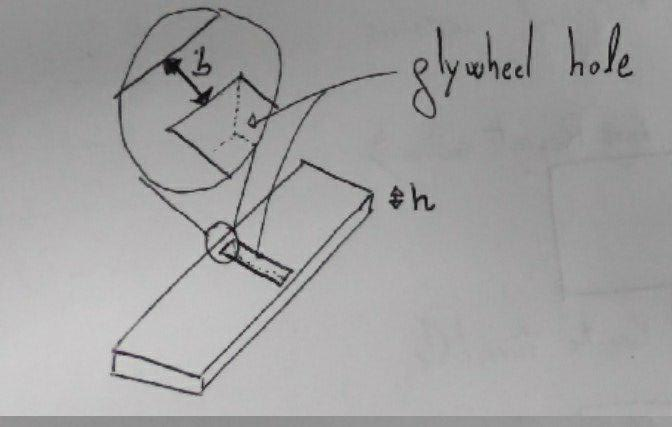
\includegraphics[width=5cm]{img/flywheel_hole.jpg}
	\caption{Flywheel hole diagram}
	\label{fig:Flywheel hole diagram}
\end{figure}
\[r_{wheel}> \sqrt{(r_{flywheel} + b)^2+\frac{h}{2}^2} + 2*\epsilon\]
\item We want to inserted the robot in to a external of diameter 0.5m so:
\begin{figure}[ht]
	\centering
	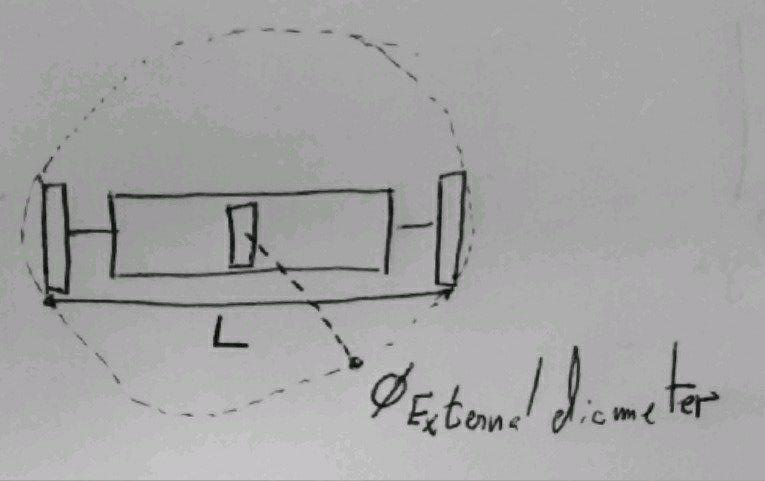
\includegraphics[width=5cm]{img/external_diameter.jpg}
	\caption{External diameter diagram}
	\label{fig:External diameter diagram}
\end{figure}
\[0.25^2 m > \sqrt{r_{wheel}^2 + L/2}\]
\item We can place all the devices:
\[L > 0.3m + w \]
\end{enumerate}

\subsection{Motor specifications}

Here we have the factory specifications of our motors: 
\begin{itemize}
    \item Operating voltage: between 3 V and 9 V
    \item Nominal voltage: 6 V
    \item Free-run speed at 6 V: 176 RPM
    \item Free-run current at 6 V: 80 mA
    \item Stall current at 6V: 900 mA
    \item Stall torque at 6V: 5 kg·cm
    \item Gear ratio: 1:35
    \item Reductor size: 21 mm
    \item Weight: 85 g
\end{itemize}

\subsection{Optimizing the design}
There are two different function we would like to maximize:
\begin{itemize}
    \item Equation \ref{Maximum angle using pendulum system}, that indicates the maximum force we can deliver at permanent state, and so limit the maximum speed:
     \[sin(\alpha_{max}) = \frac{m_{cylinder} * (r_{max}- r_{min})}{m_{total} * r_{wheel}}\]
     \item Equation \ref{Maximum angle using flywheel system}, that indicates the maximum force we can deliver at any given moment.
     \[sin(\alpha_{max}) = - \frac{\tau_{motor} (w)}{m_{total} * g * r_{wheel}} \]
\end{itemize}

In order to maximize equation \ref{Maximum angle using pendulum system}, we have decided to put only two cylinder.
By design we have that
\[r_{flywheel} = 3 * r_{cylinder}\]
\[m_{cylinder} = \rho * w * \pi * r_{cylinder}^2 \]
\[r_{max} = r_{flywheel} - r_{cylinder}\]
\[r_{min} = r_{cylinder}\]


Rewriting equation \ref{Maximum angle using pendulum system} we get:
\[sin(\alpha_{max}) = \frac{\rho * w * \pi * r_{cylinder}^2 * (r_{flywheel} - 2 * r_{cylinder})}{m_{total} * r_{wheel}}\]
\[\Rightarrow \frac{\rho * w * \pi * (\frac{1}{3} r_{flywheel})^2 * (\frac{1}{3} r_{flywheel})}{m_{total} * r_{wheel}} \]
\[\Rightarrow \frac{\rho * w * \pi * r_{flywheel}^3}{27 * m_{total} * r_{wheel}}\]

\[m_{total} = m_{rest} + N * m_{cylinder}\]


\[\Rightarrow \frac{\rho * w * \pi * r_{flywheel}^3}{(m_{rest} + N * m_{cylinder}) * 27 * r_{wheel}}\]

\[\Rightarrow \frac{\rho * w * \pi * r_{flywheel}^3}{(m_{rest} + 2 * \rho * w * \pi * r_{cylinder}^2) * 27 * r_{wheel}}\]

\[\Rightarrow \frac{\rho * w * \pi * r_{flywheel}^3}{(m_{rest} + \frac{2}{9} * \rho * w * \pi * r_{flywheel}^2) * 27 * r_{wheel}}\]

We can conclude from this equation that given a fixed $r_{flywheel}$ we want to chose the smallest $r_{flywheel}$ possible.


%%Fix $r_{wheel}$ and $r_{flywheel}$, it's clear that we will want the maximum possible 
\iffalse
The function we want to maximize is the maxim height we can reach because it has into account the maximum speed and the maximum resistance we can face.
Our hypothesis is that we start our resistance at maximum speed $\dot{y}_max$.


supposing we where travelling at the maximum velocity in plane:
\[h_{max}= - r_{wheel} * R * \dot{\theta}_{max} * (\dot{\theta}_0-\dot{\theta}_{max}) * \frac{I_{flywheel}(r)}{m_{total} * g * r_{wheel}}\]
$\dot{\theta}_{max}$ will be given by the motor specifications and we won't optimize this parameter so we can remove it.
The mass will be a constant + the mass of the flywheel which will depend linearly on $w$.
\[g= r_{wheel} * \frac{I_{flywheel}(r)^2}{m_{total} * g * r_{wheel}*(m_{total} + \frac{1}{2} *m_{wheel}) * r_{wheel}^2}\]
\[g= \frac{I_{flywheel}(r)^2}{m_{total} * g * (m_{total} + \frac{1}{2} *m_{wheel}) * r_{wheel}^2}\]
\[g= \frac{I_{flywheel}(r)^2}{m_{total} * g * (m_{total} + \frac{1}{2} *m_{wheel}) * r_{wheel}^2}\]
\[g= \frac{(6 * m_{cylinder} * r_{max}^2)^2}{m_{total} * g * (m_{total} + \frac{1}{2} *m_{wheel}) * r_{wheel}^2}\]
\[g= \frac{(6 * \rho * w * \pi * r_c^2* r_{max}^2)^2}{m_{total} * g * (m_{total} + \frac{1}{2} *m_{wheel}) * r_{wheel}^2}\]
\[g= \frac{(6 * \rho * w * \pi * (\frac{r_{flywheel}}{3})^2* (\frac{2*r_{flywheel}}{3})^2)^2}{m_{total} * g * (m_{total} + \frac{1}{2} *m_{wheel}) * r_{wheel}^2}\]
\[g= \frac{(\frac{8}{3} * \rho * w * \pi * r_{flywheel}^4)^2}{m_{total} * g * (m_{total} + \frac{1}{2} *m_{wheel}) * ((r_{flywheel} + b)^2+\frac{h}{2}^2)} + 2*\epsilon\]
\[m_{total} =6* m_{cylinder}+m_{rest} = 6 * \rho * w * \pi * r_c^2 + m_{rest} = 6 * \rho * w * \pi * (\frac{r_{flywheel}}{3})^2 + m_{rest} \]
\[m_{total} =\frac{1}{3} * \rho * w * \pi * r_{flywheel}^2 + m_{rest} \]
\[0.25 = r_{wheel}^2 + L/2\]
\[0.25 - r_{wheel}^2 =  + L/2 \Rightarrow L=2*(0.25-r_{wheel}^2) = .5-r_{wheel}^2\]
\[ L = .5-(r_{flywheel} + b)^2+\frac{h}{2}^2 \]
\[w = L - 0.3m = .5-(r_{flywheel} + b)^2+\frac{h}{2}^2 -0.3 = .2-(r_{flywheel} + b)^2+\frac{h}{2}^2\]

This plot shows how g varies when we change $R_{flywheel}$ between 0 and .5:


The maximum will be find on the border of all the restrictions?
\fi




\subsection{Hypothesis}
Assuming that the body is well balanced
